\chapter{Języki programowania dla mikrokontrolerów AVR}
\label{ch:02}

Mikrokontrolery programowalne pozwalają na budowanie zaawansowanych urządzeń wbudowanych. Wymagają one do tego języków programowania spełniających szereg wymagań m.in.: niskopoziomową manipulację sprzętem i generowanie kodu optymalnego pod kątem czasowym i pamięciowym.

\section{Mikrokontrolery AVR}
Platforma mikrokontrolerów AVR, utworzona przez firmy Atmel i aktualnie będąca własnością Microchip, jest jedną z najbardziej popularnych platform wykorzystywanych w budowaniu urządzeń wbudowanych \ksremark{Skąd wiemy, że jest najpopularniejsza? Trzeba zacytować.}. Ośmiobitowa architektura tych mikrokontrolerów powstała w roku 1996, na rynek wprowadzona została w roku 1997. Jej najważniejszymi cechami stały się prostota wytwarzania dla niej oprogramowania, niski pobór mocy oraz przystępna cena układów \ksremark{cytowanie}.

Mikrokontrolery AVR zostały oparte na ośmiobitowym procesorze RISC w zmodyfikowanej architekturze harwardzkiej z autorskim zestawem instrukcji. W zależności od rodziny rdzeń procesora może pracować z zakresie częstotliwości 1-20 MHz lub 32 MHz dla rodziny XMEGA.
W podstawowej wersji architektury, dyspozycji programisty zostały przekazane:
\begin{itemize}
\item pamięć Flash, wykorzystywana jako pamięć programu,
\item pamieć SRAM, służąca przechowywaniu zmiennych,
\item pamięć EEPROM, umożliwiająca przechowywanie dużych wartości statycznych,
\item zbiór rejestrów wewnętrznych kontrolujących pracę mikrokontrolera oraz służących do wykonywania instrukcji,
\item rejestry portów wejścia/wyjścia,
\item w zależności od modelu: liczniki zegarowe, konwertery analogowo-cyfrowe i cyfrowo-analogowe, sprzętowe interfejsy dedykowane dla protokołów tj. TWI, UART, SPI, USB, Ethernet.
\end{itemize}

Zależnie od wymagań projektowanego systemu systemu wbudowanego, dostępne jest wiele modeli mikrokontrolerów. Ze względu na ich mnogość można wyróżnić trzy najpopularniejsze podrodziny:
\begin{itemize}
\item tinyAVR -- niska cena, mała ilość pamięci oraz wyprowadzeń (od 8 do 32),
\item megaAVR -- szeroka gama rozszerzeń i funkcji, większa ilość pamięci i wyprowadzeń (od 28 do 100) względem tinyAVR,
\item XMEGA -- wyższe taktowanie procesora.
\end{itemize}

\section{Popularyzacja platformy AVR za pośrednictwem Arduino}

Prawdziwym przełomowym momentem dla platformy AVR stał się rok 2010, kiedy w trakcie wydarzenia Maker Faire w Nowym Yorku zaprezentowano nową płytkę rozwojową firmy Arduino, nazwaną Arduino UNO. Pomimo istnienia poprzedników, płytka ta stała się najpopularniejszą platformą dla początkujących elektroników. \ksremark{cytowania}

UNO ma dwa mikrokontrolery AVR \ksremark{cytowanie}:
\begin{itemize}
\item ATmega328P będący głównym mikrokontrolerem podłączonym do portów wejścia/wyjścia na płytce rozwojowej,
\item ATmega16U2 wykorzystywany jako programator USB oraz pozwalający na komunikację z głównym mikrokontrolerm poprzez port szeregowy. Po modyfikacji jego programu, możliwe jest także wykorzystanie innych trybów protokołu USB np. HID.
\end{itemize}
Użycie dwóch układów nie tylko zwiększyło możliwości płytki prototypowej. Miało także wpływ na łatwość korzystania z platformy poprzez brak wymogu instalacji sterowników dzięki protokołowi USB CDC (ang. \english{communications device class}).

Dla płytki Arduino powstało także środowisko programistyczne i zestaw bibliotek skierowany do początkujących programistów. Wyróżniają się one prostotą i przejrzystością. Edytor pozwala na kompilację kodu i programowanie płytek rozwojowych bez skomplikowanej konfiguracji. Biblioteki dla języka C, dostarczone wraz ze środowiskiem, ukierunkowane są na prostotę i czytelność kodu, ukrywając przed programistą niskopoziomowe cechy programowania systemów wbudowanych. Rysunek \ref{fig:edytor} przedstawia edytor Arduino IDE dostarcza przez firmę Arduino wraz z przykłowym programem Blink.
\begin{figure}
\centering
	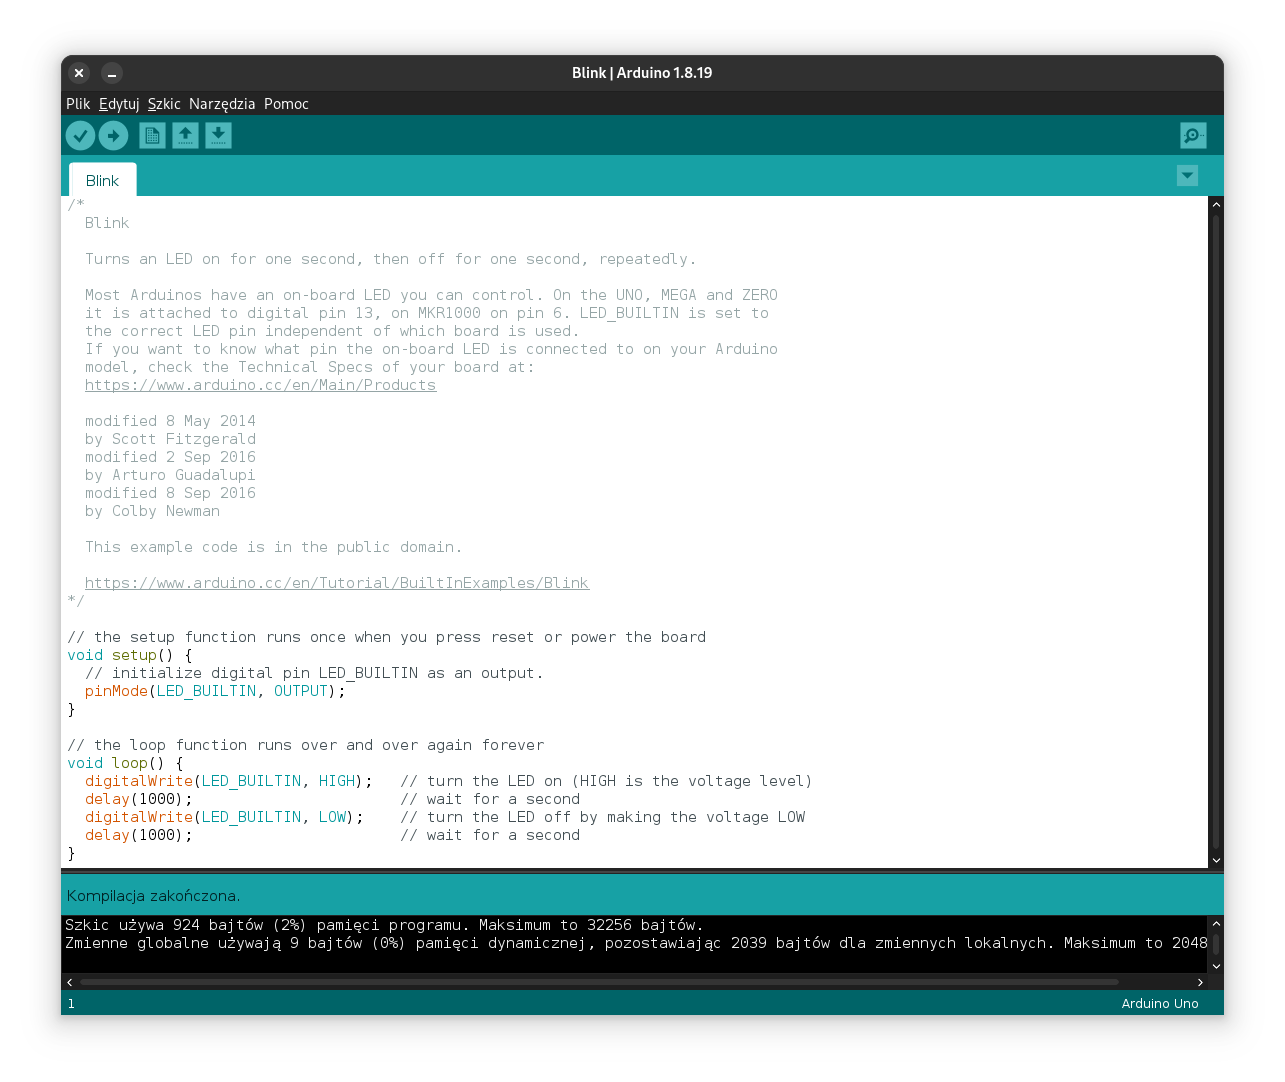
\includegraphics[width=1\textwidth]{graf/arduino-ide-blink.png}
	\caption{Edytor Arduino IDE z przykładowym programem Blink}
\label{fig:edytor}
\end{figure}

\section{Języki programowania}
Oprogramowanie wytwarzane dla systemów wbudowanych wymaga niskopoziomowego dostępu do sprzętu. Ze względu na niską ilość zasobów i jednoczesną złożoność programów pracujących na mikrokontrolerach, wykorzystuje się języki ogólnego przeznaczenia (ang. \english{general-purpose programming languages}), które pozwalają na bezpośrednią manipulację pamięcią. Oficjalnie wspieranymi językami przez środowisko programistyczne AVR są C, C++ i Assembly, dostarczanymi za pośrednictwem GNU Compiler Collection \ksremark{cytowanie}.

Wraz ze wzrostem popularności mikrokontrolerów AVR powstały także alternatywne kompilatory i interpretery dla popularnych języków programowania. Implementacje niektórych z języków można znaleźć pod nazwami:
\begin{itemize}
\item AVR-Rust -- zmodyfikowana wersja kompilatora Rust dla platformy AVR \cytowanie,
\item AVR-Ada (AVR-GNAT) -- kompilator języka Ada dla AVR \cytowanie,
\item PyMite -- minimalistyczny interpreter jezyka Python 2.5 \cytowanie,
\item NanoVM -- wirtualna maszyna dla kodu bajtowego języka Java \cytowanie.
\end{itemize}

\ksremark{Ten rozdział jest zdecydowanie za krótki.}

%\begin{itemize}
%\item sformułowanie problemu
%\item osadzenie tematu w kontekście aktualnego stanu wiedzy (\english{state of the art}) o poruszanym problemie
%\item  studia literaturowe \cite{bib:artykul,bib:ksiazka,bib:konferencja,bib:internet} -  opis znanych rozwiązań (także opisanych naukowo, jeżeli problem jest poruszany w publikacjach naukowych), algorytmów, 
%\end{itemize}
%
%
%Wzory  
%\begin{align}
%y = \frac{\partial x}{\partial t}
%\end{align}
%jak i pojedyncze symbole $x$ i $y$  składa się w trybie matematycznym.
%

%%%%%%%%%%%%%%%%%%%%%%%%



